\section{Inheritance}
Inheritance is always then used, when specific components want to be reused and extended. Inheritance can be bad because it creates a very strong dependency.

\begin{itemize}
  \itemsep -0.5em 
  \item Inheritance is default public (structs). For classes the inheritance is private.
  \item The constructors are not inherited implicitly we have to specify that.
  \item The parent is always constructed first and after that the children.
  \item Assining or send parameters per value from an inherited class to the base class result in \textbf{Object Slicing}.
\end{itemize}

\begin{lstlisting}[language=C++]
class MyClass : Base {}; // implicit private 
struct MyStruct : Base {}; // implicit public 

class MyClass : public Base {
	public:
		 using Base::Base; // inherit constructor
};
\end{lstlisting}

\subsection{Initialising Multiple Base Classes}
 Base constructors can be explicitly called in the member initializer list. You should put base class constructor class before the initialization of members. The compiler enforces this rule, even though you can put the list of initializers in wrong order.
 
 \begin{lstlisting}[language=C++]
class DerivedWithCtor : public Base1, public Base2 {
	int mvar; 
public:
	// calls base1, base2, mvar
	DerivedWithCtor(int i, int j) : Base1{i}, Base2{}, mvar{j} {}
};
\end{lstlisting}

\subsection{Dynamic Polymorphism}
\begin{itemize}
  \itemsep -0.5em 
  \item Operator and function overloading and templates allow polymorphic behaviour at compile time
  \item Basae class is required to have virtual member functions
  \item Dynamic polymorphism needs object references or (smart) pointers to work
  	\SubItem{Syntax overhead}
  	\SubItem{The base class must have a good abstratction}
  	\SubItem{Copying carries the danger of slicing (partial copying)}
\end{itemize}

\subsubsection{Shadowing Member Functions}
\begin{itemize}
  \itemsep -0.5em 
  \item if a function is reimplemented in a derived class, it shadows its counterpart in the base class
  \item However, if accessed through a declared bases object, the shadowing function is ignored
\end{itemize}

\begin{lstlisting}[language=C++]
struct Base {
	// shadowed function 
	void sayHello() const {
		"Im Base\n"
	}
}
struct Derived : Base {
	// shadowing function
	void sayHello() const {
		std::cout << "hi, im derived\n";
	}
};
void greet(Base const & base) {
	base.sayHello(); 
}
in main() {
	Derived derived{};
	greet(derived); // Hi, im Base (static call)
}
\end{lstlisting}

\subsection{Virtual Member Functions}
\begin{itemize}
  \itemsep -0.5em 
  \item To achieve dynamic polymorphism "virtual" member functions are required
  \item "Virtual" member functions are bound dynamically.
  \item The virtual keyword ist automatically inherited and does not have to be restated at childs.
  \item The sub needs to state overriding functions with "override"
  \item To override a virtual function the signatures has to be the same! (constnes included)
\end{itemize}

\begin{lstlisting}[language=C++]
struct Base {
  virtual void sayHello() const {
    std::cout << "Hi, I'm Base\n";
  }
};

struct Derived : Base {
  void sayHello() const { // virtual is automatically inhertited
    std::cout << "Hi, I'm Derived\n";
  }
};
void greet(Base const & base) {
  base.sayHello();
}

int main() {
  Derived derived{};
  greet(derived); // Hi, I'm Derived (dynamic call)
}
\end{lstlisting}

\subsection{Calling Virtual Member Functions}
\begin{itemize}
  \itemsep -0.5em 
  \item Value Object
  	\SubItem{Class type determines function, regardless of virtual}
  \item	Reference
  	\SubItem{Virtual member of derived class called through base class reference}
  \item Smart Pointer
  	\SubItem{Virtual member of derived class called through smart pointer to base class}
  \item Dump Poiner (rarely used)
  	\SubItem{Virtual member of derived class called through base class pointer}
\end{itemize}

\begin{lstlisting}[language=C++]
void greet(Base base) {
	base.sayHello(); // Value: always calls base
}

void greet(Base & base) {
	base.sayHello(); // Reference: dynamic binding
}

void greet(std::unique_ptr<Base> base) {
	base.sayHello(); // dynamic binding
}

void greet(Base const * base) {
	base->sayHello(); // dynamic binding
}
\end{lstlisting}

\subsection{Abstract Base Classes}
\begin{itemize}
  \itemsep -0.5em 
  \item There are no Interfaces in C++
  \item A pure virtual member function makes a class abstract
  \item To mark a virtual member function as pure virtual it has zero assigned after its signature
  \item Abstract classes cannot be instantiated (like in Java)
\end{itemize}

\begin{lstlisting}[language=C++]
struct abstractBase {
	virtual void doitnow() = 0;
}
\end{lstlisting}

\subsection{Destructors}
\begin{itemize}
  \itemsep -0.5em 
  \item Classes with virtual members require a virtual Destructor
  \item Otherwise when allocated on the heap with make\_unique and assigned to a unique\_ptr only the destructor of Base is called
  \item \lstinline|std::shared_ptr<T>| memorizes the actual type and knows which destructor to call.
\end{itemize}

\begin{lstlisting}[language=C++]
struct Fuel {
  virtual void burn() = 0;
  virtual ~Fuel() { std::cout << "put into trash\n" }
};

struct Plutonium : Fuel {
  void burn() { std::cout << "split core\n"; }
  ~Plutonium() { std::cout << "store many years\n"; } // automatically inherits virtual
};

int main() {
  std::unique_ptr<Fuel> surprise = std::make_unique<Plutonium>(); // both called
}
\end{lstlisting}

\subsection{Object Slicing}
Assigning or passing by value a derived class value to a base class variable/parameter incurs object slicing. Only base class member variable are transferred.

\begin{lstlisting}
struct Base {
	int member{};
	explicit Base(int initial) :
		member{initial}{} 
	virtual ~Base() = default;
	virtual void modify() { member++; } 
	void print(std::ostream & out) const;
};
struct Derived : Base {
	using Base::Base; // inherit constructor
	void modify() { member += 2; }
};
// main.cpp
void modifyAndPrint(Base base) {
	base.modify();
	base.print(std::cout); 
}
int main() {
	Derived derived{25};
	modifyAndPrint(derived);  // Output: 26
}
\end{lstlisting}


The object slicing problem can be solved if we set the copy operations as delted.
\begin{lstlisting}[language=C++]
struct Base {
	Base & operator=(Base const & other) = deleted;
	Book(Book const & other) = deleted;
}
\end{lstlisting}

\subsection{Member Hiding}
Member functions in derived classes hide base class member with the same name, even if different parameters are used. By using the base class member we can solve the problem.

\begin{figure}[h!]
  \center
  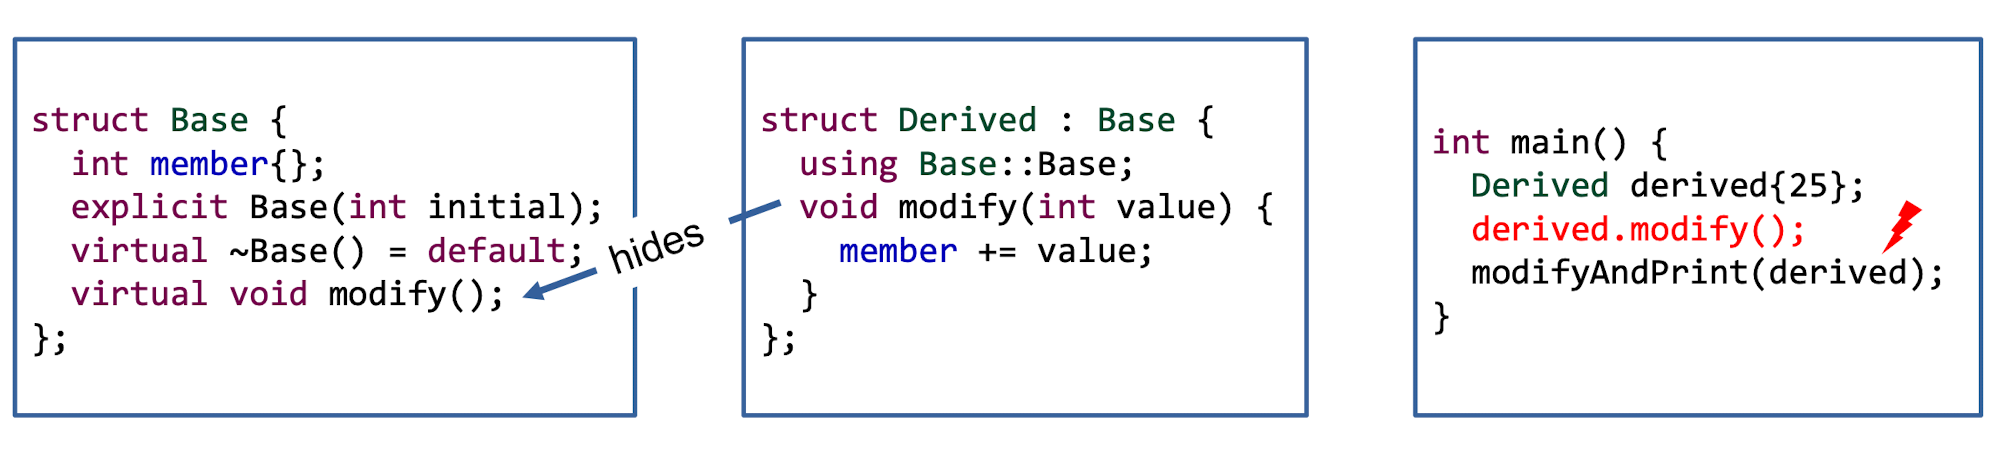
\includegraphics[width=0.75\linewidth]{memberhiding}
  \caption{Member Hiding Problem}
\end{figure}

\begin{figure}[h!]
  \center
  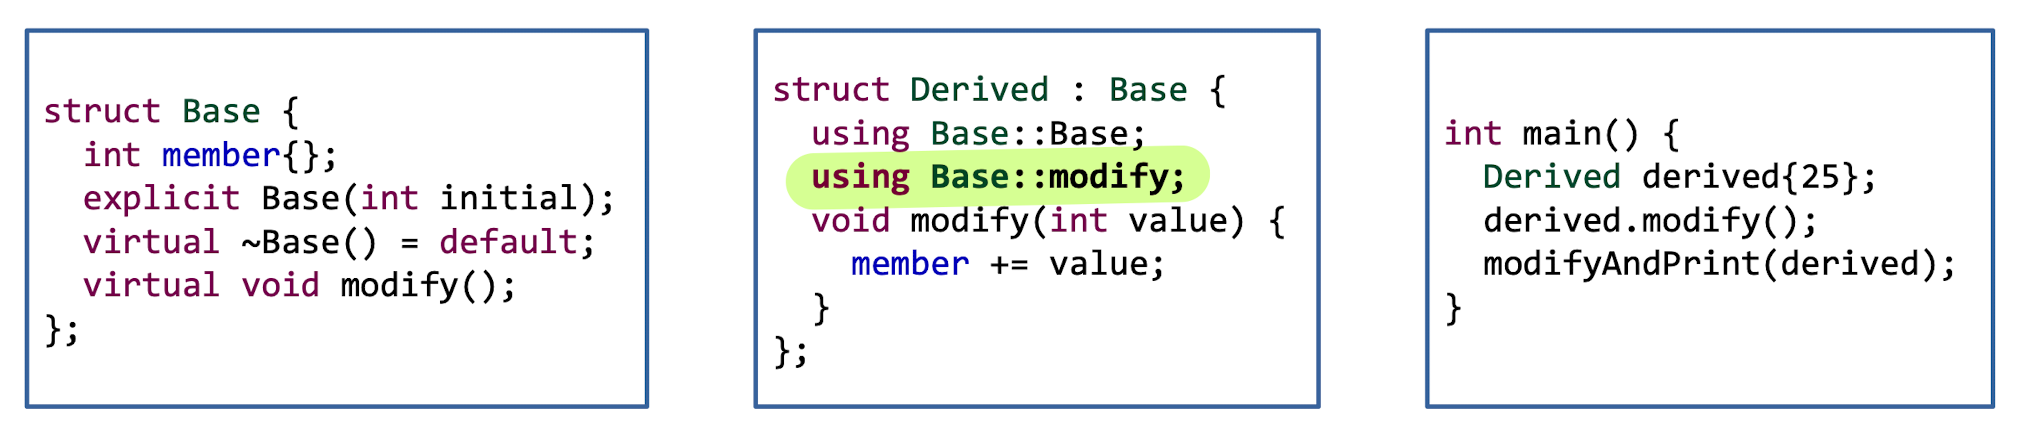
\includegraphics[width=0.75\linewidth]{memberresolution}
  \caption{Member Hiding Problem Solution}
\end{figure}






